%
% $RCSfile: double_hierarchy.tex,v $
%
% Copyright (C) 2002-2008. Christian Heller.
%
% Permission is granted to copy, distribute and/or modify this document
% under the terms of the GNU Free Documentation License, Version 1.1 or
% any later version published by the Free Software Foundation; with no
% Invariant Sections, with no Front-Cover Texts and with no Back-Cover
% Texts. A copy of the license is included in the section entitled
% "GNU Free Documentation License".
%
% http://www.cybop.net
% - Cybernetics Oriented Programming -
%
% http://www.resmedicinae.org
% - Information in Medicine -
%
% Version: $Revision: 1.1 $ $Date: 2008-08-19 20:41:06 $ $Author: christian $
% Authors: Christian Heller <christian.heller@tuxtax.de>
%

\subsection{Double Hierarchy}
\label{double_hierarchy_heading}
\index{Double Hierarchy}
\index{Whole-Part Relationship}
\index{Dialectical Relationship between Whole and Part}
\index{Conceptual Interaction}
\index{Part}
\index{Property}
\index{Constraint}

Finally, what makes up the character of a model (in the understanding of the
human mind) is a combination of two hierarchies: the \emph{Parts} it consists
of, together with \emph{Meta Information} about it.

Most properties of a molecule in \emph{Chemistry}, for example, are determined
by the number and arrangement of its atoms. \emph{Hydrogen} (H$_{2}$) becomes
\emph{Water} (H$_{2}$O) (with a totally different character) when just one
\emph{Oxygen} (O) atom is added per hydrogen molecule. The Wikipedia Encyclopedia
\cite{wikipedia} cites and writes about Richard Levins and Richard Lewontin
who, in their book \textit{The Dialectical Biologist} \cite{levins}, sketch a
\emph{dialectical} approach to biology:

\begin{quote}
    They focus on the (dialectical) relationship between the \emph{Whole} (or
    \emph{Totality}) and the \emph{Parts}: \textit{Part makes Whole, and Whole
    makes Part} \cite[p. 272]{levins}. That is, a biological system of some kind
    consists of a collection of heterogeneous parts. All of these contribute to
    the character of the whole, as in reductionist thinking. On the other hand,
    the whole has an existence independent of the parts and feeds back to affect
    and determine the nature of the parts. This back-and-forth (dialectic) of
    causation implies a dynamic process. \ldots\ Further, each species is part
    of the \emph{Environment} of all of the others.
\end{quote}

The kinds of meta information discussed in the previous sections were also
called \emph{Dimensions} or \emph{Conceptual Interaction} between a \emph{Whole}
and its \emph{Parts}. They may represent very different properties and each of
them may be constrained to certain values- or areas of validity.

\begin{figure}[ht]
    \begin{center}
        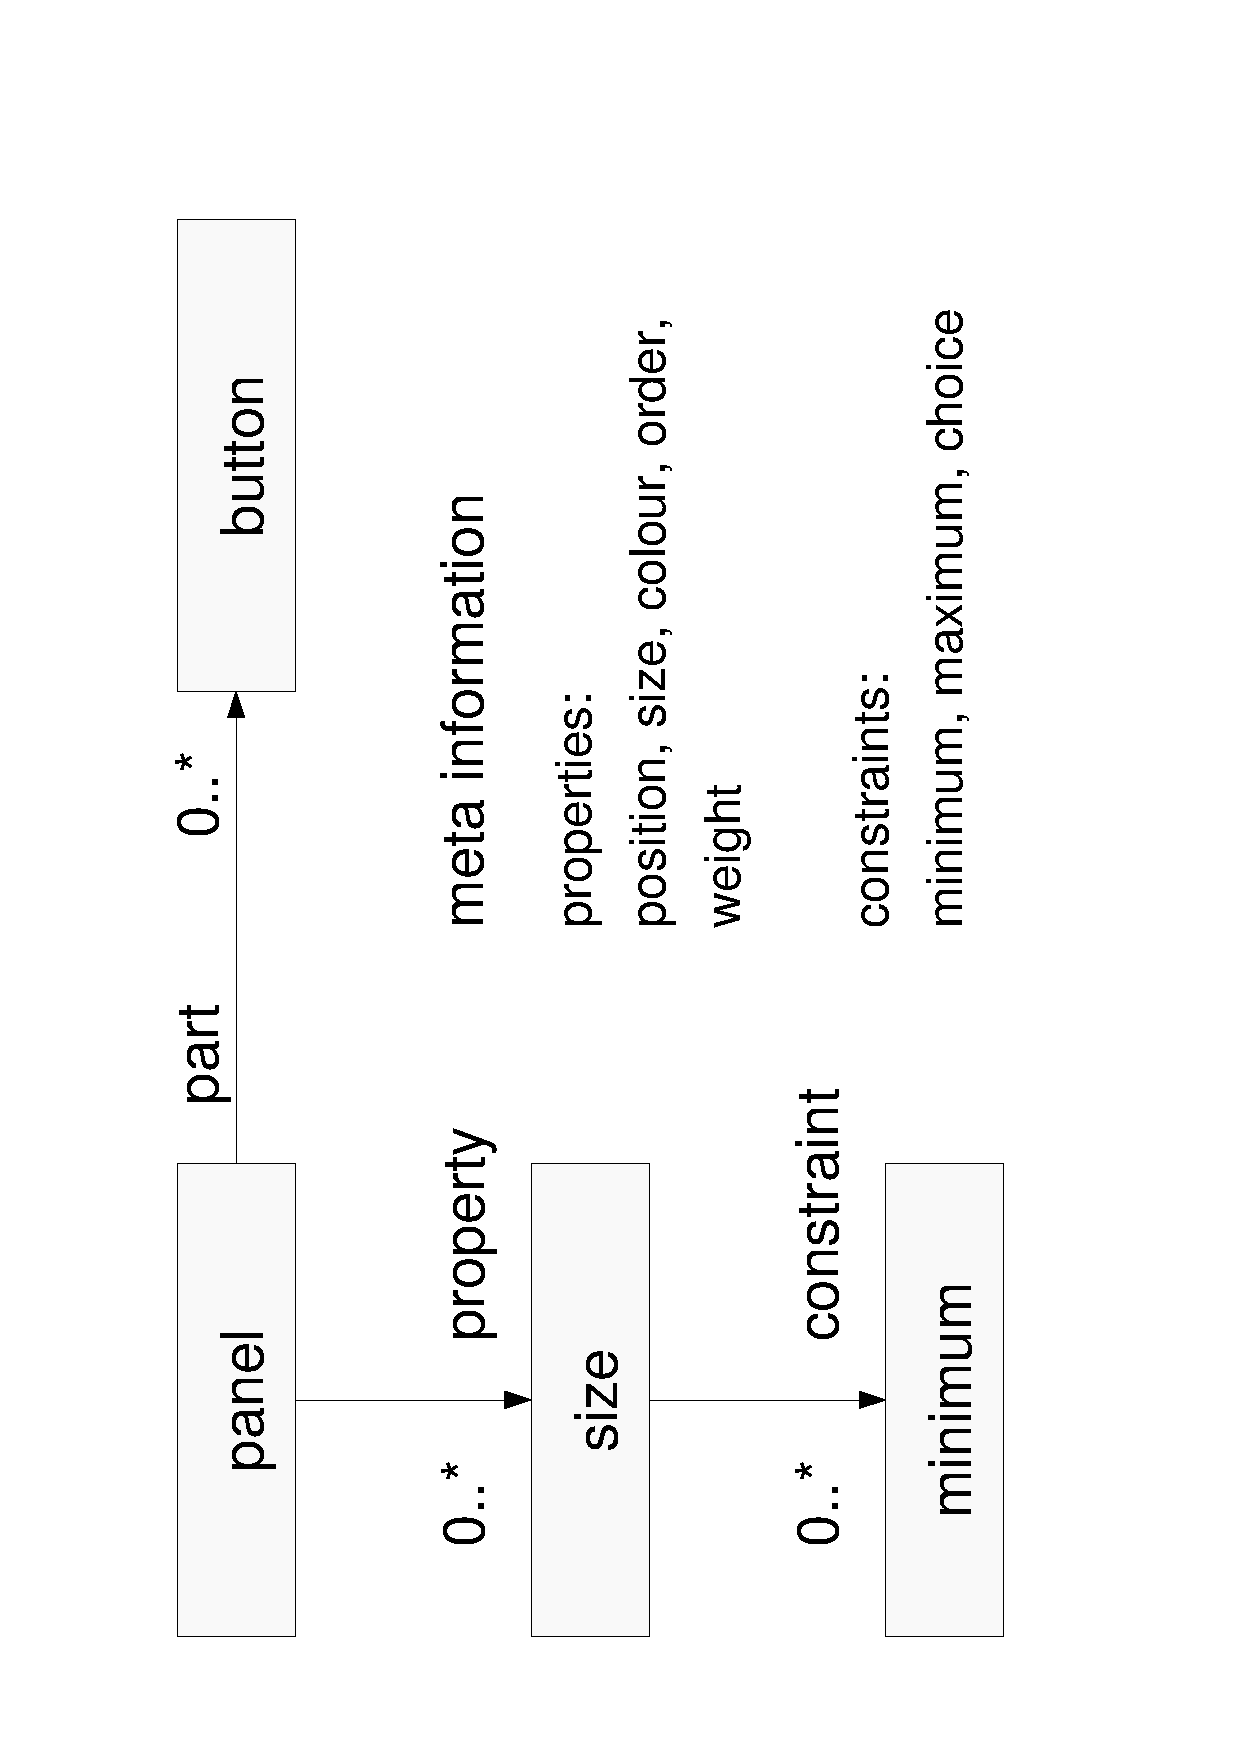
\includegraphics[scale=0.3,angle=-90]{graphic/double.pdf}
        \caption{Double Hierarchy of Parts and Meta Information}
        \label{double_figure}
    \end{center}
\end{figure}

Figure \ref{double_figure} illustrates the \emph{Double Hierarchy} here
spoken of. A graphical panel was chosen as example model. It may consist of
smaller parts, among them being a number of buttons. Altogether, they form the
\emph{Part Hierarchy}. On the other hand, there are properties like the size,
position or colour of the buttons, which are neither part of the panel, nor of
the buttons themselves; they are information \emph{about} the buttons and form
an own \emph{Meta Hierarchy}. To the latter do also belong constraints like the
minimum size of a button or a possible choice of colours for it. Constraints can
be treated like meta information about properties. Once again: \emph{Properties}
are information about a \emph{Part}; \emph{Constraints} are information about a
\emph{Property}.
